\title{Signalverarbeitung auf dem STEMlab}

% English Version:
%\team{%
%    Raphael Frey,\\
%    \hspace*{6.85em}Noah H\"usser}
%
%%\client{Important Client}
%
%\coaches{%
%    \hspace*{2.015em}Prof. Dr. Richard Gut,\\
%    \hspace*{6.85em}Michael Pichler}
%
%\expert{\hspace*{3.025em}Dr. J\"urg Stettbacher}

% Deutsch:
\team{%
    Raphael Frey,\\
    \hspace*{7.46em}Noah H\"usser}

%\client{Important Client}

\coaches{%
    \hspace*{2.625em}Prof. Dr. Richard Gut,\\
    \hspace*{7.35em}Michael Pichler}

\expert{\hspace*{3.037em}Dr. J\"urg Stettbacher}

\fssummary{
    Dieses Projekt realisiert ein System zur Messung von analogen Signalen vom
    Kilohertz- bis in den unteren  Megahertz-Bereich. Dazu wird ein Red Pitaya
    STEMlab zur  Erfassung und Verarbeitung  des Signals und ein  Computer zur
    Visualisierung verwendet.
}

\fsgraphics{
    \centering
    \vspace{1.5em}
    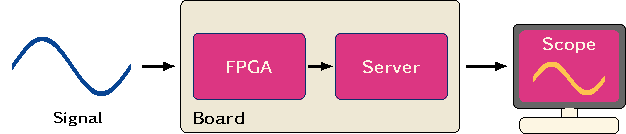
\includegraphics[width=0.8\textwidth]{images/p6fhu-intro-system-overview.pdf}
    \vspace{1em}
}

\fscontent{
    \section{Idee}
    Ziel ist, teure Laborger\"ate wie  Oszilloskop und Spectrum Analyzer durch
    eine  g\"unstigere  L\"osung  zu  ersetzen. Daf\"ur wird  ein  Red  Pitaya
    STEMlab mit integriertem FPGA verwendet.

    \begin{center}
        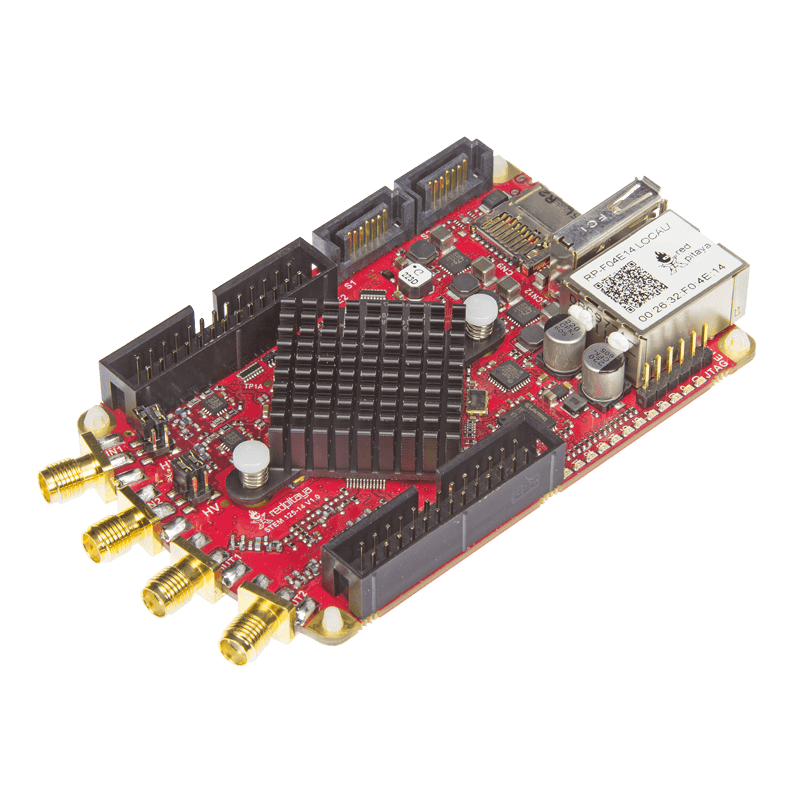
\includegraphics[width=0.3\textwidth,clip=true,viewport=1cm 3cm 20cm 17.5cm]{images/p6fhu-stemlab125-14-photo.png}
        \footnotesize Red Pitaya STEMlab\\ \textcolor{gray}{(Quelle: elektor.com)}
    \end{center}

    %\newcol
    \section{Konzept}
    Zur Übertragung  via Netzwerk  m\"ussen die Daten  aus dem  ADC dezimiert
    werden. F\"ur  diesen   Zweck  implementiert  dieses  Projekt   ein  neues
    Filtersystem  sowie eine  neue Applikation  zur Visualisierung  der Daten.
    Die Filter sind  als Kaskaden auf dem FPGA  des STEMlab implementiert. 

    Die   grafische    Darstellung   erfolgt   via    Web-Applikation,   womit
    Kompatibilit\"at \"uber verschiedene Plattformen erreicht wird.

    \begin{minipage}{0.32\textwidth}
        \begin{center}
            \vspace{3ex}
            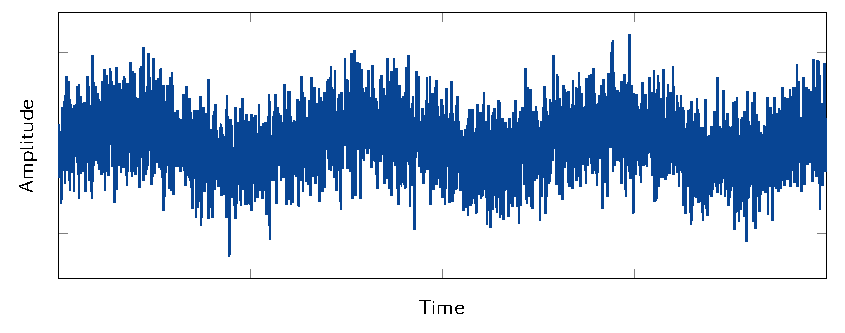
\includegraphics[width=\textwidth]{images/p6fhu-noisySine.pdf}
            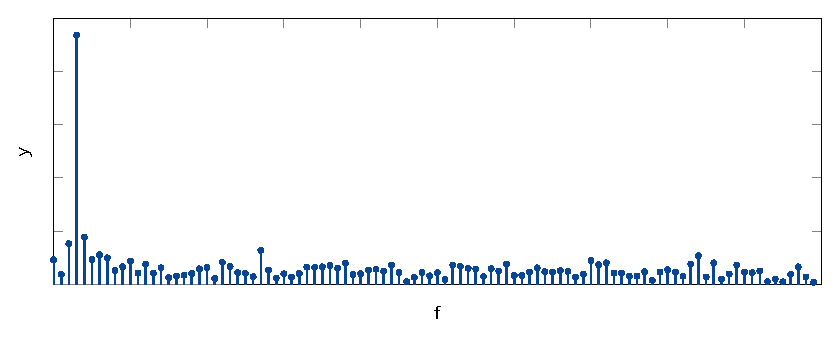
\includegraphics[width=\textwidth]{images/p6fhu-noisySineFFT.pdf}
            \footnotesize{Zeit- und Frequenzbereich vor Durchlauf der Filterketten}
            \vspace{4ex}

            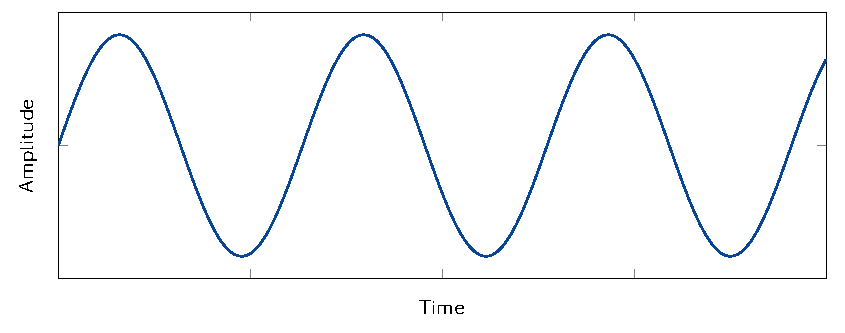
\includegraphics[width=\textwidth]{images/p6fhu-sine.pdf}
            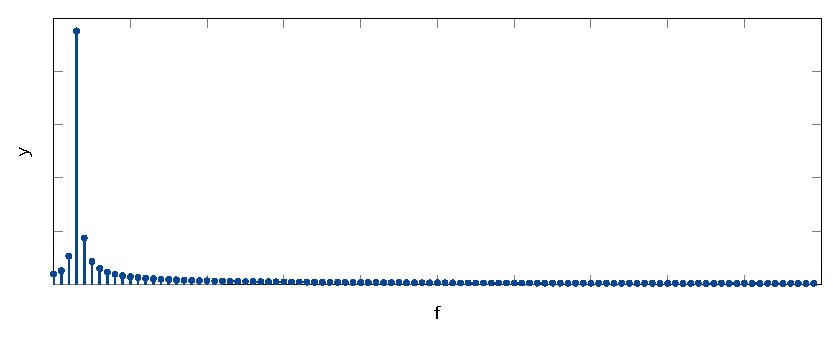
\includegraphics[width=\textwidth]{images/p6fhu-sineFFT.pdf}
            \footnotesize{Zeit- und Frequenzbereich nach Durchlauf der Filterketten (vereinfacht)}
        \end{center}
    \end{minipage}

    %\newcol
    \section{Resultat}
    Es  sind sechs  Dezimationsketten vorhanden,  welche Abtastraten  zwischen
    \SI{50}{\kHz} und  \SI{25}{\MHz} erlauben. Wichtige  Einstellungen können
    direkt aus der Applikation im Browser vorgenommen werden.

    Die Software  erlaubt sowohl den  direkten Export  von Daten als  auch die
    Anbindung  von Dritt-  Applikationen f\"ur  besondere Anforderungen.   Das
    gesamte Projekt ist Open Source, womit bei Bedarf weitere \"Anderungen und
    Erg\"anzungen vorgenommen werden k\"onnen.

    \vspace{4ex}
    \begin{center}
        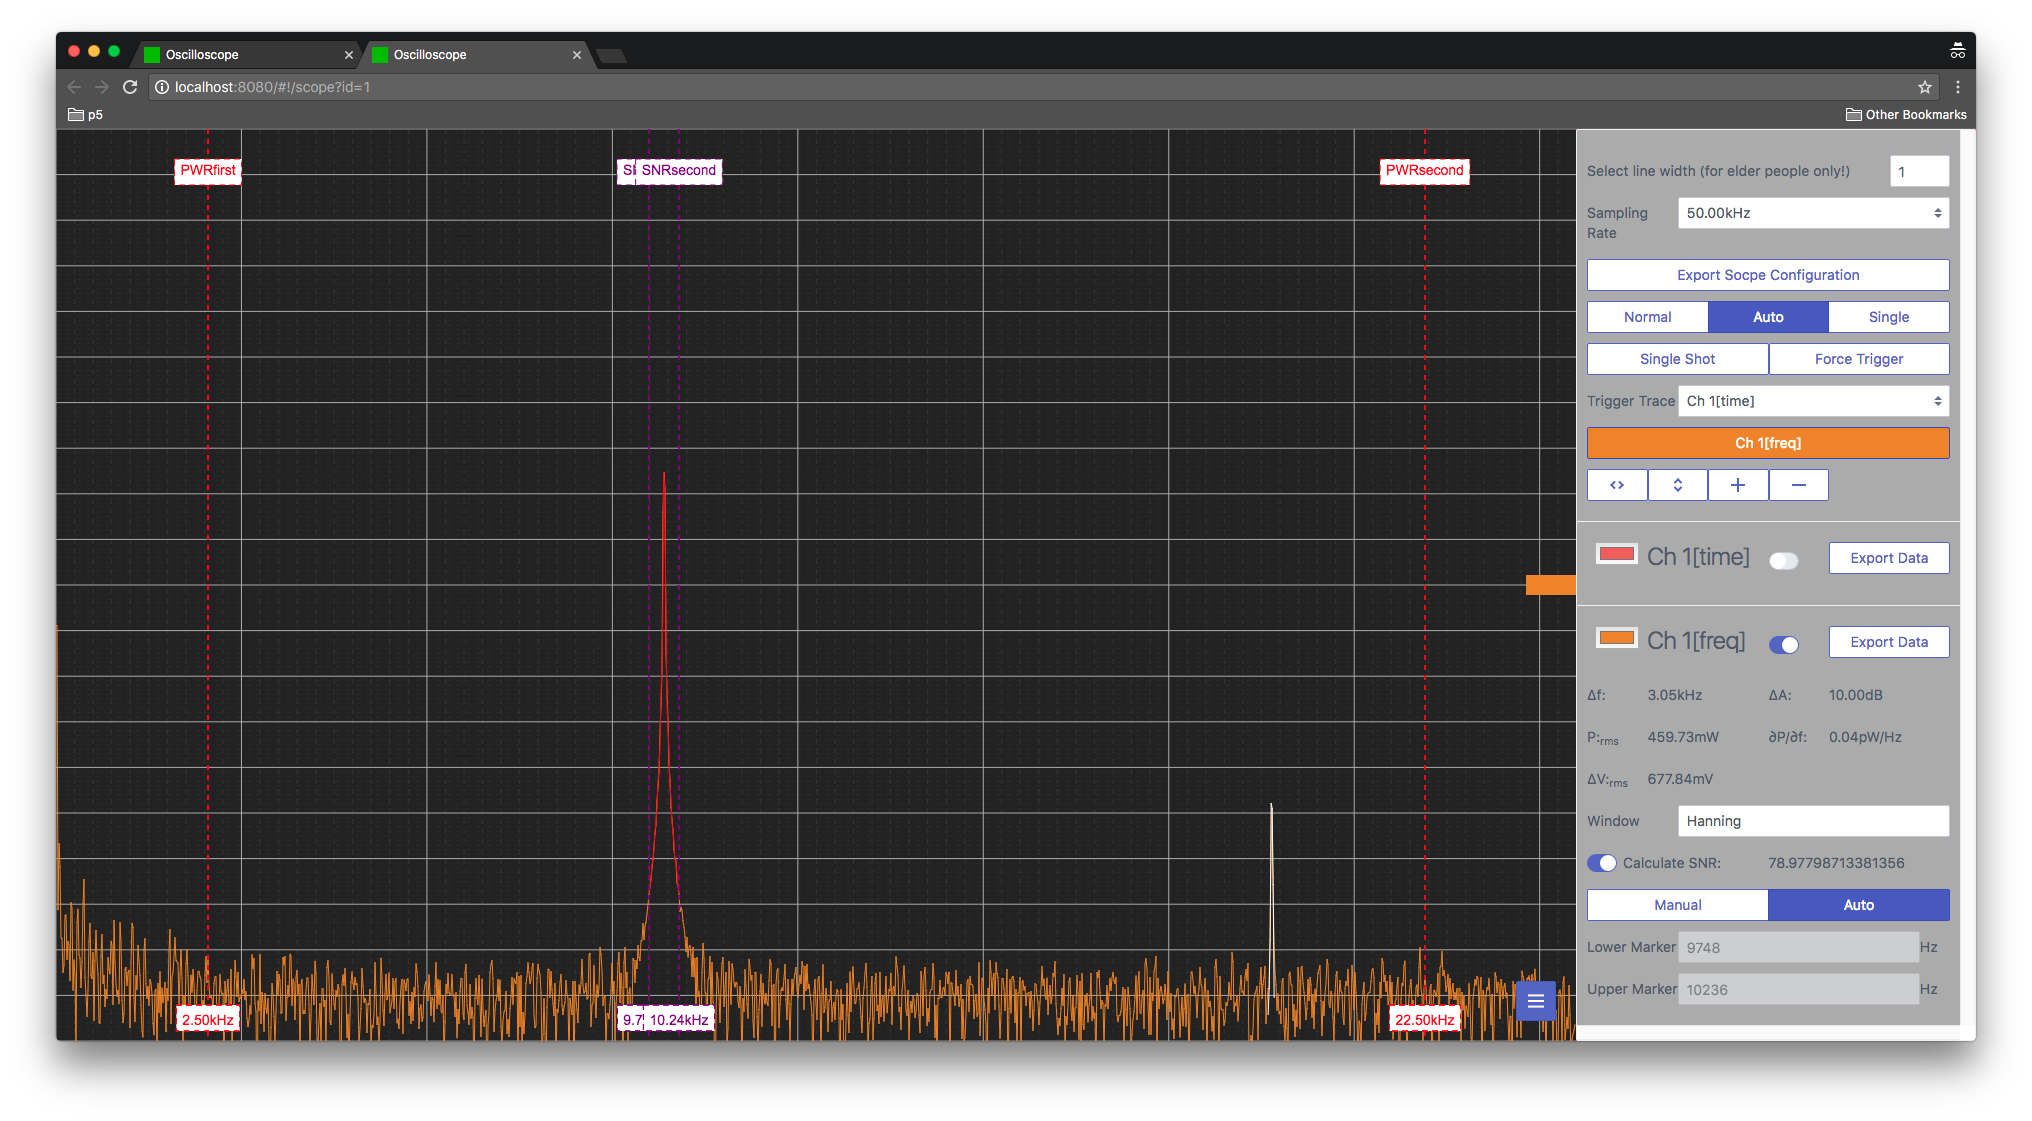
\includegraphics[width=0.32\textwidth]{images/p6fhu-scope.png}
        \footnotesize{Screenshot des Oszilloskops}
    \end{center}
}

\infobox{Eckdaten}{%
    \begin{description}
        \item[Filter-Typen:] FIR und CIC
        \item[Sampling-Frequenzen Ausgang:] sechs Stufen zwischen und \SI{50}{\kHz} \SI{25}{\MHz}
        \item[D\"ampfung im Stopband:] minimum \SI{60}{\dB}
        \item[SNR:] bis \SI{84}{\dB}, je nach Signal und Filterkette
        \item[Link:] \url{https://github.com/alpenwasser/pitaya}
    \end{description}
}
